\subsubsection{View}

\begin{figure}[H]
\centering
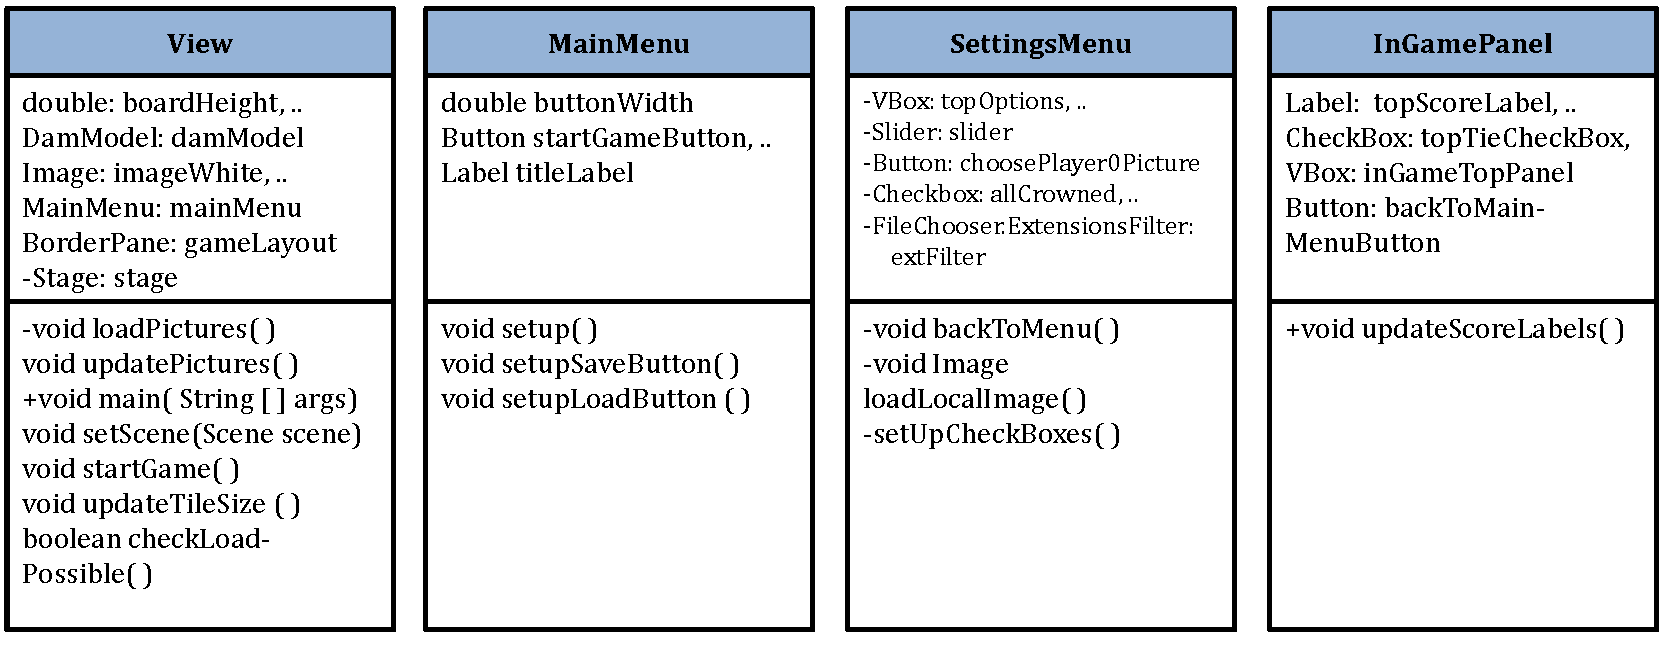
\includegraphics[width = 1.0  \textwidth]{Figurer/classesView.pdf}
\caption{Klassediagram over de klasser der bliver brugt i View-delen af MVC designmønstret.}
\label{fig:classesView}
\end{figure}

%   RR
%\item Hvordan startes spillet? (method calls)
\textbf{Spil startes:} 
Det første der sker når programmet startes, er at de forskellige scener bliver sat op og main menu scenen (\texttt{mainMenuScene}) bliver hæftet til \texttt{JavaFX Applications}'s \texttt{Stage}. I hver scene hæftes de brugte Layouts og modeller. Da \texttt{mainMenuScene} er den første aktive scene, startes spillet altså i main menuen. Derfra har man fri adgang til indstillinger og spillet selv. Ved at trykke på \texttt{"Start new game"} knappen bliver \texttt{gameScene} gjort aktivt og spillet startes med de valgte indstillinger (eller standard indstillinger hvis intet er valgt). \\

Knappen \texttt{"Start new game"} kører metoderne \texttt{startGame}, \texttt{setScene(gameScene)} og \texttt{resetValues} fra henholdsvis \texttt{View} og \texttt{Control} klasserne, hvilket sørger for at spil modellen dannes, spillets scene vises og nødvendige in-game værdier bliver nulstillet. På den måde er knappens funktion uafhængig af om den trykkes når spillet startes, eller efter adskillige spil, da modellen altid startes på ny. 

\begin{figure}[H]
\centering
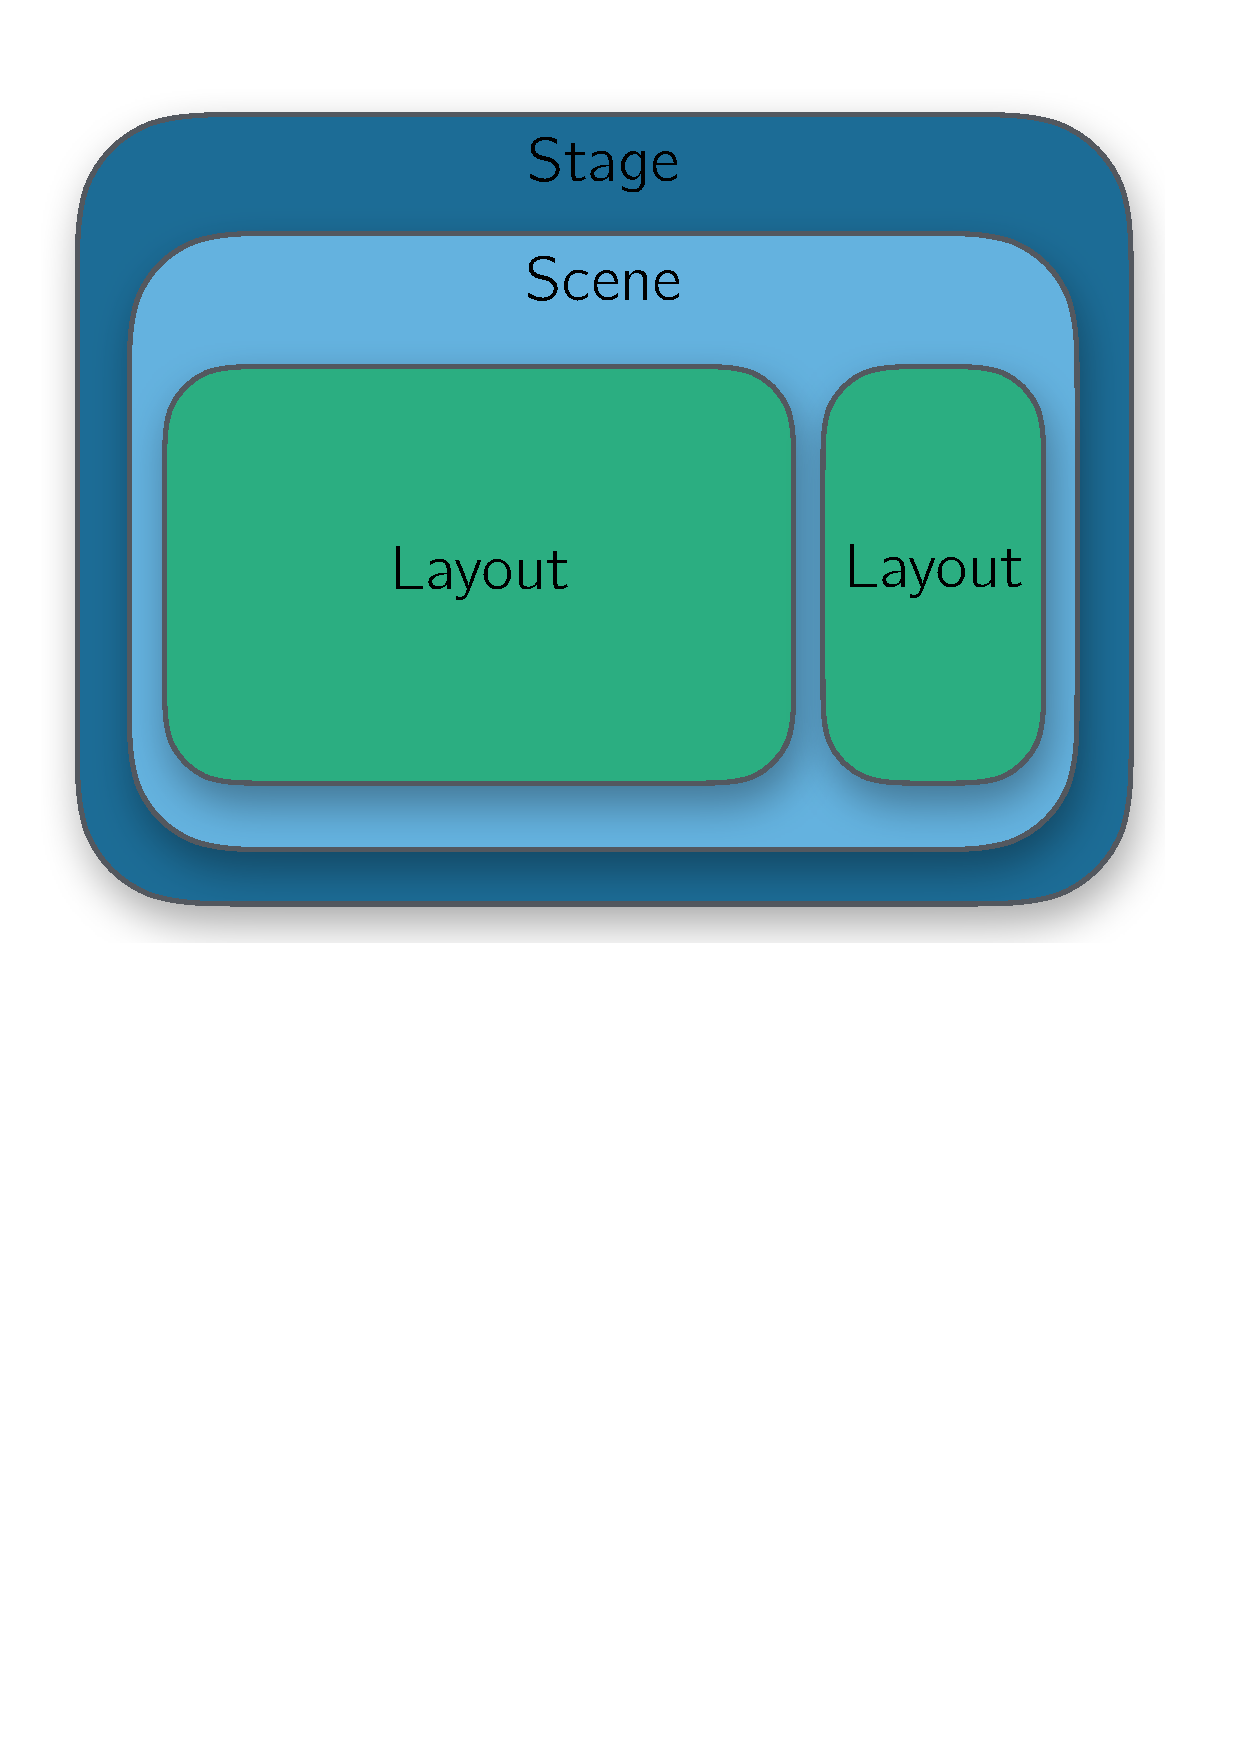
\includegraphics[width = 0.5\textwidth]{Figurer/GUI.pdf}
\caption{Forhold mellem Stage, Scene og Layout i JavaFX.}
\label{fig:GUI}
\end{figure}

%   RR
%\item Hvordan håndteres brug af scenes?    
\textbf{Scenes:} 
Vi bruger følgende scenes: \texttt{mainMenuScene}, \texttt{settingsScene} og \texttt{gameScene}. Hver scene repræsenterer et segment af programmet, og for at skifte fra fx menuen med indstillinger til main menu, skiftes fra \texttt{settingsScene} til \texttt{mainMenuScene} direkte i \texttt{JavaFX Applications}'s \texttt{Stage} via \texttt{stage.setScene(mainMenuScene)}. Scenen kan også fra andre klasser ved brug af \texttt{View.setScene(Scene scene)}.\\

%Jens
%Hvordan bruges I styles og CSS?
\textbf{Cascading Style Sheets:} Stilen og udseende af de tre forskellige scener: \texttt{gameScene}, \texttt{settingsScene} og \texttt{mainMenuScene}, bliver sat af tre korresponderende \texttt{.css} filer med tilsvarende navne via fx \texttt{.getStyleSheets().add("GameScene.css")}. Ved brug af stylesheets bliver bla. skriftyper og størrelser, baggrundsfarve, tekstfarve mm. indstillet. Syntaksen og formen af \texttt{.css} filer gør det nemt at ændre hele sceners udseende hurtigt og bidrager til høj fleksibilitet og overskuelighed til programmets udseende. CSS er især brugbart til større programmer.\\

%Jens
%Hvordan håndteres user input?
\textbf{Bruger input:} Al interaktion med brugeren af programmet håndteres gennem listeners som sætter gang i forskellige events. \texttt{JavaFX} har som standardindstilling listeners til piletasterne og mellemrum aktiveret. Dette gør menunavigering nemmere, da mellemrum bla. sætter gang i et \texttt{setOnKeyPressed()} event for en markeret knap, og piletasterne skifter mellem hvilken knap der er markeret. Udover dette har vi gjort brug af fire yderligere forskellige slags listeners. Den første er tilføjet til \texttt{gameScene} og \texttt{settingsScene}; en \texttt{setOnKeyPressed} listener der, hvis den trykkede knap er Esc, skifter den viste scene ud med hovedmenuen. De sidste tre er til museinteraktionenerne pressed, dragged og released, som bliver brugt til at flytte brikker. Disse listeners aktiveres i \texttt{Piece}-klassens konstruktør under metoden \texttt{move}.
\begin{lstlisting}
void move() {
    setOnMousePressed(mouse -> {
        startThisPiece(this);
    });
    setOnMouseDragged(mouse -> {
        updateThisPiece(this, mouse);
    });
    setOnMouseReleased(mouse -> {
        if (hasLegalEndPosition(this)) {
            finishThisPiece(this);
            startNextTurn();
        } else {
            continueThisPiece(this);
    	}
        updateAllPieces();
        updateAllTiles();
        runAI();
    });
}
\end{lstlisting}
De kaldte metoder ovenfor findes i \texttt{Control} og \texttt{TopLevelControl}. \\

% Magnus
% Hvordan skiftes mellem billeder af ikke-fokus brik, valgt brik, og kronet brik? (adv)
\textbf{Skift af billeder (valgt, kronet):} Når en brik trækkes med musen eller krones, opdateres brikkens billede. I \texttt{TopLevelControl} findes metoden \texttt{updateThisPiece}, der køres når en brik trækkes:
\begin{lstlisting}
static void updateThisPiece(Piece piece, MouseEvent mouse) {
// If not crowned, change between normal and chosen 
if (!piece.getCrowned()) {
piece.setFill(piece.player == Player.Upper ? blackChosen : whiteChosen); } } }
\end{lstlisting}

\texttt{blackChosen} og \texttt{whiteChosen} er \texttt{ImagePatterns} i \texttt{View} klassen, der repræsenterer billederne i figur \ref{fig:defaultPieces}.  \\

%% MIKKEL %%
% GULD RING???????
\textbf{Guld ring:} Guld ringen, der indikerer om en brik er kronet, sættes på to forskellige måder. Hvis en brik bliver kronet i sin konstruktør, bliver kantfarven sat til guld via fieldet \texttt{crownedColor}. Når en brik når til modstanderens bageste række, bliver brikken kronet via metoden \texttt{finishThisPiece}. Et eksempel på dette er: 

\begin{lstlisting}
if (selectedPiece.player == Player.Upper && releasedAtY == tileAmount - 1) {
	selectedPiece.setCrowned(true);
	selectedPiece.setFill(View.blackCrowned);
	selectedPiece.setStroke(Color.GOLD);
}
\end{lstlisting}

%% MIKKEL %%
% Hvordan er rød og guld ring implementeret?
\textbf{Rød ring:} Når en brik slippes, køres metoden \texttt{updateAllPieces}. \texttt{updateAllPieces} kører en række andre metoder, nogle af hvilke vil blive beskrevet nedenfor.

\begin{enumerate}
    \item Metoden \texttt{checkPossibleKills} hvis \texttt{mandatoryFirstKill} er sat til. \texttt{checkPossibleKills} kører et loop over alle brikker i \texttt{pieces}, og kører metoden \texttt{canKill} på dem.
    
    \item \texttt{canKill} tager imod et \texttt{Piece} og tjekker, om brikken kan dræbe i hver af de retninger der er tilgængelige for den gennem metoden \texttt{canKillThisDirection}.
    
    \item \texttt{canKillThisDirection} tager imod et \texttt{piece}, samt modelkoordinater \texttt{dx} og \texttt{dy}, der betegner hvilke koordinater der skal tjekkes, relativt til brikkens egne modelkoordinater. \texttt{canKillThisDirection} returnere en boolean, der er sand hvis der er en brik på feltet betegnet gennem \texttt{dx} og \texttt{dy}, hvor den fjendtlige brik er af et andet hold en den valgte brik, samt at feltet efter den fjendtlige brik er ledigt. 
    
    \item Hvis alle disse er sande, returnerer \texttt{canKillThisDirection} sand, og sætter \texttt{canKill} til true på den valgte brik gennem metoden \texttt{setCanKill}. 
    
    \item \texttt{setCanKill} tager en boolean som argument, og hvis denne er true, sætter den brikkens \texttt{stroke} til rød, gennem fieldet \texttt{killColor}. Hvis den tager imod boolean false, sætter den enten brikkens stroke til guld, hvis den er kronet, ellers sætter den stroke til transparent.
   
\end{enumerate}

% Magnus
% Hvordan animeres spawn og død? 
\textbf{Animation af spawn\footnote{Med begrebet spawn menes: Hændelsen hvor en ny brik bliver placeret på brættet.} og død:} Animationen af spawn og død er implementeret ved brug af \texttt{ScaleTransition}. Animationen sker når der skiftes scene. Brikker bliver markeret som kronet ved at deres \texttt{isCrowned} field opdateres, så animationen sker ikke, når brikker krones; det er samme brik. Animation af død er implementeret i klassen \texttt{DamModel}, da det er integreret i \texttt{removePiece} metoden, der først skalerer brikken ned (visualiserer død), derefter fjerner brikken fra dens tilhørende \texttt{tile} (via \texttt{setPiece(null)}), endeligt fjernes den visuelt fra skærmen via \texttt{getChildren().remove(piece)}.

\begin{figure}[H]
\centering
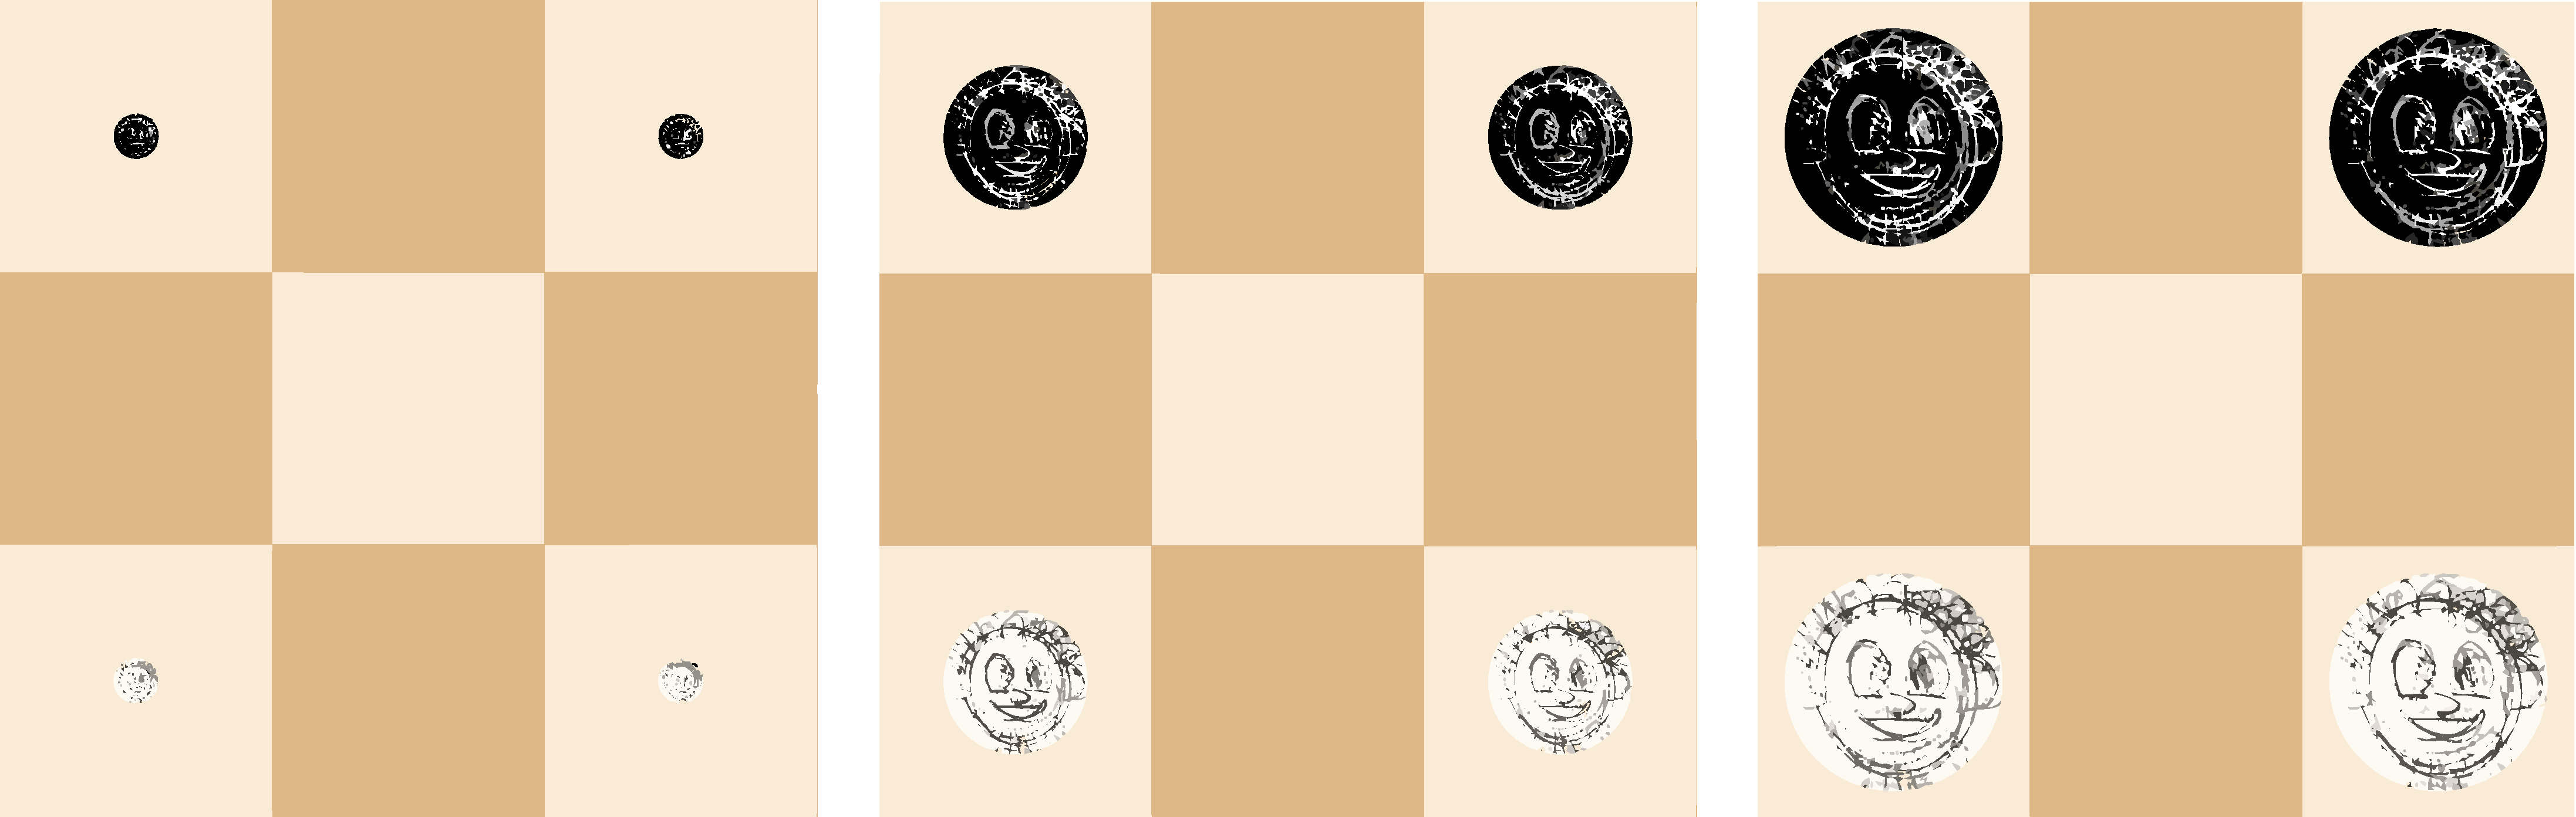
\includegraphics[width = 0.8  \textwidth]{Figurer/spawn.pdf}
\caption{Animation af hvordan brikker spawnes på brættet. Brikkerne skaleres fra et punkt op til deres aktuelle størrelse over et forløb på 600 millisekunder.}
\label{fig:spawn}
\end{figure}

